\documentclass[]{article}
\usepackage{lmodern}
\usepackage{amssymb,amsmath}
\usepackage{ifxetex,ifluatex}
\usepackage{fixltx2e} % provides \textsubscript
\ifnum 0\ifxetex 1\fi\ifluatex 1\fi=0 % if pdftex
  \usepackage[T1]{fontenc}
  \usepackage[utf8]{inputenc}
\else % if luatex or xelatex
  \ifxetex
    \usepackage{mathspec}
  \else
    \usepackage{fontspec}
  \fi
  \defaultfontfeatures{Ligatures=TeX,Scale=MatchLowercase}
\fi
% use upquote if available, for straight quotes in verbatim environments
\IfFileExists{upquote.sty}{\usepackage{upquote}}{}
% use microtype if available
\IfFileExists{microtype.sty}{%
\usepackage{microtype}
\UseMicrotypeSet[protrusion]{basicmath} % disable protrusion for tt fonts
}{}
\usepackage[margin=1in]{geometry}
\usepackage{hyperref}
\hypersetup{unicode=true,
            pdftitle={A national, multi-decadal, water color and landsat dataset},
            pdfauthor={Matthew Ross and lots of others!},
            pdfborder={0 0 0},
            breaklinks=true}
\urlstyle{same}  % don't use monospace font for urls
\usepackage{graphicx,grffile}
\makeatletter
\def\maxwidth{\ifdim\Gin@nat@width>\linewidth\linewidth\else\Gin@nat@width\fi}
\def\maxheight{\ifdim\Gin@nat@height>\textheight\textheight\else\Gin@nat@height\fi}
\makeatother
% Scale images if necessary, so that they will not overflow the page
% margins by default, and it is still possible to overwrite the defaults
% using explicit options in \includegraphics[width, height, ...]{}
\setkeys{Gin}{width=\maxwidth,height=\maxheight,keepaspectratio}
\IfFileExists{parskip.sty}{%
\usepackage{parskip}
}{% else
\setlength{\parindent}{0pt}
\setlength{\parskip}{6pt plus 2pt minus 1pt}
}
\setlength{\emergencystretch}{3em}  % prevent overfull lines
\providecommand{\tightlist}{%
  \setlength{\itemsep}{0pt}\setlength{\parskip}{0pt}}
\setcounter{secnumdepth}{0}
% Redefines (sub)paragraphs to behave more like sections
\ifx\paragraph\undefined\else
\let\oldparagraph\paragraph
\renewcommand{\paragraph}[1]{\oldparagraph{#1}\mbox{}}
\fi
\ifx\subparagraph\undefined\else
\let\oldsubparagraph\subparagraph
\renewcommand{\subparagraph}[1]{\oldsubparagraph{#1}\mbox{}}
\fi

%%% Use protect on footnotes to avoid problems with footnotes in titles
\let\rmarkdownfootnote\footnote%
\def\footnote{\protect\rmarkdownfootnote}

%%% Change title format to be more compact
\usepackage{titling}

% Create subtitle command for use in maketitle
\newcommand{\subtitle}[1]{
  \posttitle{
    \begin{center}\large#1\end{center}
    }
}

\setlength{\droptitle}{-2em}
  \title{A national, multi-decadal, water color and landsat dataset}
  \pretitle{\vspace{\droptitle}\centering\huge}
  \posttitle{\par}
  \author{Matthew Ross and lots of others!}
  \preauthor{\centering\large\emph}
  \postauthor{\par}
  \predate{\centering\large\emph}
  \postdate{\par}
  \date{17 August, 2018}

\usepackage{booktabs}
\usepackage{longtable}
\usepackage{array}
\usepackage{multirow}
\usepackage[table]{xcolor}
\usepackage{wrapfig}
\usepackage{float}
\usepackage{colortbl}
\usepackage{pdflscape}
\usepackage{tabu}
\usepackage{threeparttable}
\usepackage[normalem]{ulem}

\begin{document}
\maketitle

{
\setcounter{tocdepth}{2}
\tableofcontents
}
\section{Introduction}\label{introduction}

Since the beginning of the Landsat missions, the limnologists,
oceanographers, and hydrologists have been interested in developing
universal algorithms for extracting water quality information from
remotely sensed images (Holyer 1978,Ritchie, Schiebe, and McHENRY
(1976),Maul and Gordon (1975),Klemas, Borchardt, and Treasure
(1973),Clarke, Ewing, and Lorenzen (1970)). Since these early efforts
there has been almost fifty years of work with the basic goal of using
spectral information to predict water quality parameters like total
suspended solids (TSS), Chlorophyll a (Chl.a), colored dissolved organic
matter, and secchi disk depth (SDD). However, progress towards universal
algorithms and unified approaches has been slow (Bukata
2013,Blondeau-Patissier et al. (2014),Gholizadeh, Melesse, and Reddi
(2016)), with most papers published focusing on developing predictive
methods as opposed to using predictions to interrogate process that
control water quality dynamics {[}Topp2018{]}. Much of this slow
evolution in methods and approaches comes from the inherent optical
complexity of inland waters, where spectral signatures are the result of
a complex mixture of inorganic sediment, organic sediment, algae,
dissolved organic matter, and other constituents. Compared to oceanic
remote sensing of water quality which benefits from robust, shared
datasets of \emph{in-situ} data paired with satellite overpass
reflectance (Blondeau-Patissier et al. 2014,Bukata (2013)), progress on
inland water algorithms is further impeded by the lack of a shared
overpass dataset.

Such data could go a long way towards, if not the holy -grail of
universal predictive algorithms, at least towards more unified
approaches tested on a universal dataset. Here, we create and share the
largest such overpass dataset ever assembled for inland waters by using
Google Earth Engine (Gorelick et al. 2017) Landsat archive data from
1984-2018 with data from the Water Quality Portal (E. K. Read et al.
2017) and phase one of the ``lake multi-scaled geospatial and temporal
database (LAGOSNE)''(Soranno et al. 2017) for the conterminous USA and
Alaska. Joining these datasets provides us with an unprecedented
resource to model, predict, and understand the long-term and large-scale
dynamics of variation in four key water clarity constituents: TSS, SDD,
Chl.a, and dissolved organic carbon (DOC). We also outline and share our
approach, code, and intermediate data for bringing these three free
datasets together; generating a high-graded analysis-ready dataset for
remote sensors of water quality.

\subsection{Parameter description?}\label{parameter-description}

Wondering if this deserves it's own section or just a reference to
Topp2018. For now I'm assuming that this will be explicitly cast as sort
of partB to that paper, and I am not writing out detailed explanations,
but can easily add this section.

\section{Methods}\label{methods}

\subsection{Data source description}\label{data-source-description}

Combining \emph{in-situ} data with Landsat reflectance information first
requires a large repository of water quality samples, which increases
the likelihood that a given sample happened to be taken on the same day
as a Landsat overpass. For this paper, we focused on two databases of
water quality. The first, the Water Quality Portal (WQP) has tens of
millions of water observations in all types of inland surface waters,
but there is no entity that harmonizes and cleans the data for quality
(E. K. Read et al. 2017). The second dataset we used, LAGOS, currently
only covers lakes in the northeastern United States, with plans to
expand and cover lakes across the entire USA (Soranno et al. 2017).
While LAGOS has less data than the WQP, a group of dedicated researchers
has spent years combing through the data and ensuring data quality,
making it a more analysis-ready dataset (Soranno et al. 2017). These
similar but contrasting datasets, one with more quantity (WQP) and the
other with more quality assurances (LAGOS), ensures that our dataset
covers the broadest possible number of waterbodies with the option of
limiting analyses to only the highest quality subset.

\subsubsection{Water Quality Portal}\label{water-quality-portal}

The WQP is the largest dataset of water observations ever assembled with
more than 290 million observations at 2.7 millions sites mostly in the
USA, with data dating back more than a century (E. K. Read et al. 2017).
The WQP continuously gathers water quality information from more than
450 organizations including academic, government, NGO, tribal, and state
datasets (E. K. Read et al. 2017). These datastreams are gathered and
distributed in a standardized format, making analysis across different
collection methods more readily available. Yet, the diversity of data
sources and variation in meta-data quality brings about some significant
challenges to directly using the WQP as a analysis-ready dataset
(Sprague, Oelsner, and Argue 2017). Instead end-users of the data must
carefully harmonize data across sampling methods, analytic approaches,
and units. The nature of harmonizing such large, distributed data
generates a necessary trade-off between a deep, time-consuming
exploration of data interoperability and a more shallow less
time-consuming but potentially more error-prone data quality check.

\subsubsection{LAGOS-NE}\label{lagos-ne}

The LAGOS project was, in part, meant as a direct way to address some of
the problems inherent to the WQP, with the explicit goal of building a
publically available high-quality dataset for continental-scale lake
analyses (Soranno et al. 2017). In addition to pairing \emph{in-situ}
lake data with physical lake characteristics and local geologic setting,
LAGOS researchers standardized key water quality measurements across the
87 water quality datasets that they gathered (Soranno et al. 2017). In
it's current form, the LAGOS dataset covers only lakes in the northeast
and midwest, two lake-rich regions of the USA. LAGOS provides an
end-member dataset of the highest quality for matching \emph{in-situ}
data to Landsat overpasses.

\subsubsection{Landsat}\label{landsat}

For this project, we join these two \emph{in-situ} datasets with the
Landsat data archive for Landsat missions 5, 7, and 8. The Landsat
missions started in July 1972, as the Earth Resources Observation
Satellite with an explicit mission to provide solutions for some of
earth's pressing issues associated with industry and environmental
change (Loveland and Dwyer 2012). For this project we are only using the
three most recent Landsat mission datasets: Landsat 5 with coverage from
1984-2012 and over 192745 available images; Landsat 7 which is still
collecting data after launching in July of 1999 with 190976 images; and
finally Landsat 8 which launched in November, 2013 still adding to its
collection of 61255 images. Generally, these satellites complete a full
imaging of the globe every sixteen days, except for the most polar
regions (Loveland and Dwyer 2012,Wulder et al. (2016)), meaning that for
most of the USA, a given spot will be imaged at least every sixteen
days, and-when two missions are running at the same time- every eight
days. All three satellites use different imagers to collect spectral
information in the visible and infrared wavelengths.

\subsection{Data integration}\label{data-integration}

For this project, we wanted to emphasize not only the possibilities that
come with open data, but also the importance of reproducible science and
code. In this case uniting these three distinct datasets requires a
combination of computational approaches and an architecture that allows
for a single workflow to pull data from LAGOS, the WQP, and the Landsat
archive. Despite such disparate data sources, an ideal overarching
approach allows us to break the various data pulls, munging, and joining
into seperate pieces that can be updated only as needed. Here we chose
to use a ``MAKE'' like environment (Feldman 1979) that only executes
sections of code that have been altered or when data sources are out of
date. Though this project uses three different programs R, Python, and
Google Earth Engine, all of these various languages are called directly
from R and RMarkdown files. This reliance on R makes
\href{https://github.com/richfitz/remake}{remake} an excellent choice to
keep track of changes to the complex commands required to make this
dataset. Remake is simply an R specific MAKE-like environment that can
check if code has been updated and then update all downstream
dependencies. We hope that these efforts will make recreating or
altering our specific approach easier. At a high level, all of this
architecture is meant to do something fairly simple captured by figure
\ref{fig:fig1}, joining \emph{in-situ} data to Landsat reflectance.

\begin{figure}
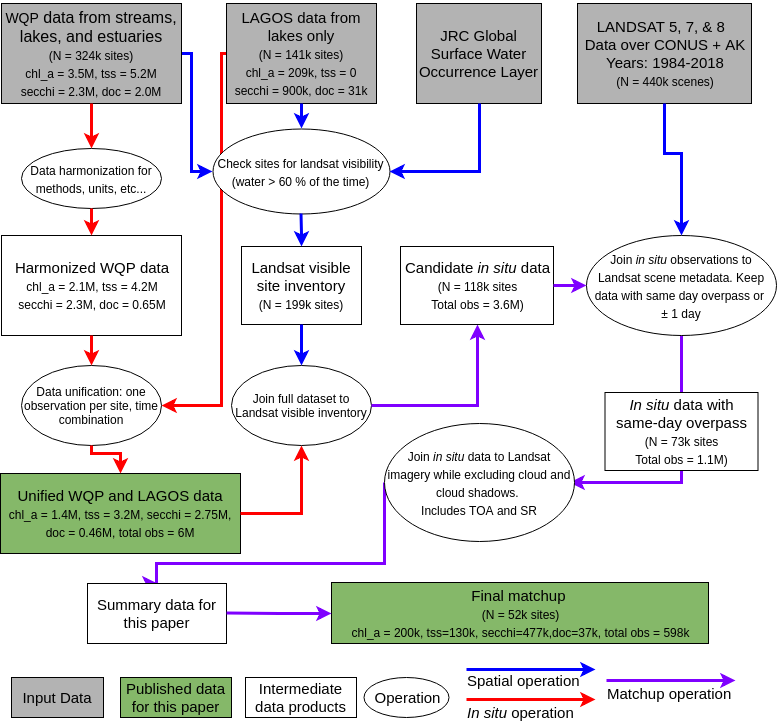
\includegraphics[width=1\linewidth]{/home/matt/Dropbox/UNC-PostDocAll/aquasat/9_report/src/Watersat_Drop_flow} \caption{Overview of data sources, steps taken to join data, and total observation counts}\label{fig:fig1}
\end{figure}

\subsubsection{\texorpdfstring{\emph{In situ} data pull and quality
control.}{In situ data pull and quality control.}}\label{in-situ-data-pull-and-quality-control.}

In this paper we focused on gathering water quality measurements that
capture the dominant controls on water clarity, these include:
Chlorophyll a (chl.a), dissolved organic carbon (DOC), and total
suspended solids (TSS). Together these three constituents combine to
control total water clarity which is captured by secchi disk depth
measurements, the fourth and final parameter we pulled for these
analyses. For the WQP we used the
\href{https://github.com/USGS-R/dataRetrieval}{dataRetrieval} package.
DataRetrieval, a package maintained and supported by the USGS, allows
for programattically downloading data from the WQP. The WQP contains
hundreds of possible paramater types (called ``characteristicName'' in
the WQP), and we carefully selected those that best represented our
target parameters based on our own expertise and previously published
research using the same data sources(E. G. Stets and Strieg 2012,Butman
et al. (2016)). The characteristicName's that we pulled are shown in
table \ref{tab:table1}. For all parameters, we pulled data for all US
states. The WQP classifies water body types in many possible categories
and we pulled data for the four following water body types: Lake,
Reservoir, Impoundment; Stream; Estuary; Facility. Finally, we only
gathered data that was reported to have been sampled in ``Water'' as a
sample media (no sediment or benthic samples).

Working with the LAGOS-NE data (version 1.087.1) required many less
decisions to combine parameters since LAGOS researchers have already
harmonized and combined parameters into simple categories that reflect
our general parameter codes(Soranno et al. 2017). LAGOS includes lake
data for: DOC, Chlorophyll a, and secchi disk depth, but no data on TSS.
As with the WQP the dataset can be simply loaded using an R package
(`LAGOSNE')(Soranno et al. 2017). This clean dataset requires very
little data cleaning and was essentially preserved as a direct product
from the LAGOSNE dataset, in sharp contrast to the much more intensive
data cleaning required to use the WQP data.

\rowcolors{2}{gray!6}{white}

\begin{table}

\caption{\label{tab:table1}Table shows the characterstic names used in our water quality portal data pull.}
\centering
\begin{tabular}[t]{>{\raggedright\arraybackslash}p{2cm}|>{\raggedright\arraybackslash}p{13cm}}
\hiderowcolors
\hline
\textbf{Parameter} & \textbf{WQP Names}\\
\hline
\showrowcolors
cdom & Colored dissolved organic matter (CDOM)\\
\hline
chlorophyll & Chlorophyll; Chlorophyll A; Chlorophyll a; Chlorophyll a (probe relative fluorescence); Chlorophyll a (probe); Chlorophyll a - Periphyton (attached); Chlorophyll a - Phytoplankton (suspended); Chlorophyll a, corrected for pheophytin; Chlorophyll a, free of pheophytin; Chlorophyll a, uncorrected for pheophytin; Chlorophyll b; Chlorophyll c; Chlorophyll/Pheophytin ratio\\
\hline
doc & Organic carbon; Total carbon; Hydrophilic fraction of organic carbon; Non-purgeable Organic Carbon (NPOC)\\
\hline
secchi & Depth, Secchi disk depth; Depth, Secchi disk depth (choice list); Secchi Reading Condition (choice list); Secchi depth; Water transparency, Secchi disc\\
\hline
tss & Total suspended solids; Suspended sediment concentration (SSC); Suspended Sediment Concentration (SSC); Total Suspended Particulate Matter; Fixed suspended solids\\
\hline
\end{tabular}
\end{table}

\rowcolors{2}{white}{white}

Turning data from the WQP into an analysis-ready dataset similar to
LAGOS-NE requires a chain of decisions that is extensively documented in
the supplemental \href{link}{website}. We have attempted to make these
decisions both clear and justifiable, with the end goal of having
parameters meet several criteria. First, all observations were verified
to ahve analytical methods that matched their parameter name, if this
were not the case samples were dropped. For example, if an observation
was supposed to report TSS, and the analytical method was ``Nitrogen in
Water,'' then that sample would be dropped. For TSS in particular, we
assumed that the terms Suspended Sediment Concentration reflected
essentially the same data despite some methodoligical differences in the
data as shown
\href{https://water.usgs.gov/osw/pubs/WRIR00-4191.pdf}{here}. Second,
all parameters were checked to make sure that the parameter name that
was downloaded, matched the actual parameter of interest. For example,
if we downloaded ``Dissolved Organic Carbon'' data, but the parameter
name in the data was ``Total Organic Carbon'' then we would drop those
samples. Third, we harmonized the data across units such that TSS and
DOC data are in mg/L, Chl.a data is in \(\mu g/L\), and secchi disk
depth is in meters. If units were nonsensical (secchi in mg/L), then we
would drop those observations. Finally, we forced both the LAGOS-NE and
the WQP data to have only one observation per datetime X site
combination. We did this by either removing true duplicates (where the
value was the same for multiple observations), averaging multiple
observations to a single observation if the coefficient of variation was
less than 0.1, and throwing out observations with too many simultaneous
observations (5 per date time combination) or too much variation with no
metadata explaining the repeat observations. We used a similar procedure
for the data that did not have timestamps and only had date information,
these data without timestamps were set to observations at noon for
matching to Landsat dates. Figure \ref{fig:fig1}. captures how these
data cleaning procedures cut out observations and sites.

While our data quality control included many checks to ensure data
quality, we also consciously avoided some other data quality assurance
steps because including them would have thrown out the majority of the
WQP data. For example, some samples included sampling depth information,
which is particularly important when matching water quality data to
reflectance information, but so few samples included depth information,
that we elected to simply keep all the data, assuming that the majority
of the data was collected near the surface (see supplement for
justification of this assumption). Some of these decisions included: not
filtering data based on sampling method, not including temperature data
as a filter for DOC and Chl.a samples, and including data that had
unlabeled sample fraction metadata. We know that some of these decisions
may not match the requirements of other research, so we have included
code and data that would allow future researchers to choose different
data quality criteria and recreate a similar, more strict dataset.

\subsubsection{\texorpdfstring{Joining \emph{in-situ} data to
Landsat}{Joining in-situ data to Landsat}}\label{joining-in-situ-data-to-landsat}

Both the WQP and LAGOS-NE datasets come with site information that
includes latitude and longitude. Joining the \emph{in-situ} data to
Landsat requires using this location data to select sites, gather
spatially averaged reflectance, and match water quality data
observations to simultaneous overpasses. For the location data, we
encounter an interesting difference in philosophy, where the WQP records
locations at the site of the observation and LAGOS-NE records location
as the center of the lake under observation. This means that if data is
both in the WQP portal and in LAGOS-NE, then we will potentially have
different reflectance information for the same water quality
observation. We kept both of these data sources, so that data users can
choose which data source best suits their needs.

The first step in linking these datasets is finding out which water
bodies are likely to be Landsat visible, where the 30m resolution pixels
of Landsat detect an unspoiled (entirely water) pixel. We elected to
only keep sites that are not only classified as water some of the time,
but are generally classified as water throughout the Landsat archive
record, using an 80\% threshold on the Pekel occurrence layer (Pekel et
al. 2016). Pekel and others (2016) used the Landsat archive to generate
a global map of how often a given pixel was classified as water from
1985-2015. For our purposes we only kept sites that were within 150
meters of at least one pixel with a water occurence of at least 60\%.
All such sites were kept in the dataset and were sptially joined to an
inventory of landsat overpass path and row, where each site was then
affiliated with a specific landsat tile.

We then generated a dataset that included information on the exact date
and time that any of the three Landsat missions imaged a given tile.
This data was then joined to the \emph{in-situ} observation data by
date. If multiple observations were taken on the same day, we kept only
the observation that was closest in time to the landsat overpass. In
order to maximize the size of the dataset, we also shouldered the
\emph{in-situ} data by one day, allowing for data to be collected
\(\pm\) one day of an overpass. This one-day shouldering is relatively
conservative for previous work in lakes (Olmanson, Brezonik, and Bauer
2011,Torbick et al. (2013)) and rivers (Griffin et al. 2011), but is
likely too permissive for estuaries and rivers with rapidly changing
discharge, where water clarity characteristics vary on sub-hour
intervals ({\textbf{???}}). The timing difference between overpasses and
\emph{in-situ} collection is preserved in the final dataset and users
can specify minimum overpass timing if they choose to be more strict.

With this trimmed down dataset of Landsat-visible sites matched to
Landsat overpass times, we used Google Earth Engine to pair
\emph{in-situ} observations with Landsat reflectance values. Landsat 5
and 7 have onboard imagers that collects seven bands of imagery centered
on three visible wavelengths (blue, green, and red) and four infrared
(near infrared, shortwave infrared 1, shortwave infrared 2, and thermal
band). Landsat 8 has the same bands with slightly different wavelengths
and improved spectral accuracy (Barsi et al., 2014) plus a few extra
bands that we did not include in this work. Landsat 7 and 8 have
panchromatic bands at 15m resolution, while landsat 5 does not. For our
matchup data, the bands we used their wavelengths and resolution are in
table \ref{tab:landsat}.

\rowcolors{2}{gray!6}{white}

\begin{table}

\caption{\label{tab:landsat}Landsat spectral summary}
\centering
\begin{tabu} to \linewidth {>{\raggedright}X>{\raggedright}X>{\raggedright}X>{\raggedright}X>{\raggedright}X}
\hiderowcolors
\hline
\textbf{Bands} & \textbf{L5 Wavelengths} & \textbf{L7 Wavelengths} & \textbf{L8 Wavelengths} & \textbf{Resolution (m)}\\
\hline
\showrowcolors
Blue & 0.45-0.52 & 0.45-0.52 & 0.452-0.512 & 30\\
\hline
Green & 0.52-0.60 & 0.52-0.60 & 0.533-0.590 & 30\\
\hline
Red & 0.63-0.69 & 0.63-0.69 & 0.636-0.673 & 30\\
\hline
Near Infrared (nir) & 0.77-0.90 & 0.77-0.90 & 0.851-0.879 & 30\\
\hline
Shortwave Infrared 1(swir1) & 1.55-1.75 & 1.55-1.75 & 1.566-1.651 & 30\\
\hline
Shortwave Infrared 2 (swir2) & 2.09-2.35 & 2.09-2.35 & 2.107-2.294 & 30\\
\hline
Panchromatic & NA & 0.52-0.9 & 0.503-0.676 & 15\\
\hline
\end{tabu}
\end{table}

\rowcolors{2}{white}{white}

At each site, we generated a 150m buffer around the site. Within this
buffered zone, we throw out any pixel that is not classified as water at
least 70\% of the time in the landsat archive (Pekel et al. 2016). All
of the Landsat data comes with quality assessment bands that indicate if
individual pixels are likely taken of land, water, clouds, aerosols,
etc\ldots{} We used these bands to throw out any pixels that were
classified as cloud and cloud shadows, but we elected to keep all data
classified as land, ice, or water, since very high sediment
concentrations can lead to classification as water or ice (Xiao cite?).
In addition to these steps, we also created a 30m buffer around the
TIGER road
\href{https://www.census.gov/geo/maps-data/data/tiger.html}{dataset}
from the US Census office, all pixels that were within 30m of any
transport artery (road, traintracks, etc\ldots{}) was removed. Once
these extra steps were taken for removing pixels that would likely spoil
the reflectance signal coming from the water, we took a spatial median
of all remaining pixels in the buffer zone for all bands. This step
leaves us with a ``wide'' (Wickham 2014) dataset with the \emph{in-situ}
observation values in columns arranged with reflectance values from
landsat for the same site X date combination.

One of the most critical components of inland water remote sensing is
the atmospheric correction, where radiance at the satellite sensor is
corrected to radiance from the land surface. Atmospheric correction,
when properly applied can correct for aersol interference, sun glint,
and other processes that might alter the radiance leaving waterbodies,
giving a much cleaner signal of the optical qualities of water. There
are many options for atmospheric correction algorithms, but Google Earth
Engine only houses the USGS Surface Reflectance archive which uses a
version of the 6S radiative transfer model called LEDAPS for Landsat 5
and 7 and different algorithm for Landsat 8 called LaSRC that uses the
ultra blue band to correct for aersols. Because the Google Earth Engine
archive only houses this one atmospheric correction approach, we pull
both the USGS surface reflectance and the uncorrected top-of-atmosphere
reflectance. Ideally this allows end users to use their best judgement
for which product is best suited to their needs. At the end of this long
chain of decisions, and operations, we are left with a matchup of
dataset of nearly 600,000 matchups between \emph{in-situ} data and
Landsat reflectance. As far as we know this is the largest such dataset
for inland water quality and some of it's summary features are described
below. \emph{THIS PARAGRAPH NEEDS CITATIONS}.

\begin{center}\rule{0.5\linewidth}{\linethickness}\end{center}

\section{Results}\label{results}

As figure \ref{fig:fig1} shows, matching data to landsat overpasses
generally reduced the total available data for a given paramter by 6-25
times, with the biggest dropoff in TSS observations and the most
retained with secchi disk depth. This intuitively makes sense, as most
TSS observations are made in streams which aren't Landsat visible, while
secchi observations are mostly in lakes, which are visible. As a result
of this steep dropoff we elected to drop CDOM from the pipeline because
there were only 2761 CDOM results in the entire WQP before any data
cleaning. The remaining data is well distributed across the parts of the
USA with many lakes and rivers in the Upper Midwest, Northeast, and
Florida, with notable data concentrations near the Chesepeake Bay and
along the U.S. East Coast in major estuarine environments (Fig
\ref{fig:map}). The western United States has notably less data
available, which likely reflects both much lower concentrations of lakes
and rivers, and potentially a bias in the completeness of the WQP
towards certain states.

\begin{figure}
\centering
\includegraphics{aquasat_outline_files/figure-latex/map-1.pdf}
\caption{\label{fig:map} Distribution of observations across the
conterminous USA. The data is split by observation type, where total
represents an overpass for any of the four primary parameters}
\end{figure}

As is evident in the spatial distribution of data shown in figure
\ref{fig:map}, lakes dominate the matchup dataset contributing 76.5\% of
the data to the entire dataset, most of that coming from the secchi
data. Beyond the general trends of what regions are best represented in
the data, it is useful to know the number of observations at a given
site. Figure \ref{fig:distribution} shows the breakdown of overpasses at
a given site and it highlights an important caveat to this dataset. The
vast majority of sites have less than ten matchups, making it unlikely
that one can rely on a single site to build, test, and validate a model
that uses reflectance to predict water quality parameters. However,
there are thousands of sites with at least one observation and if these
sites are close, share the same waterbody or drainage basin, one may be
able to borrow information across sites to have enough data for
modelling/prediction applications. Algthough the majority of sites have
only one overpass, there are several hundred for each parameter that
have at least 50 overpasses, which presents exciting opportunities for
site-specific remote water quality predictions.

\begin{figure}
\centering
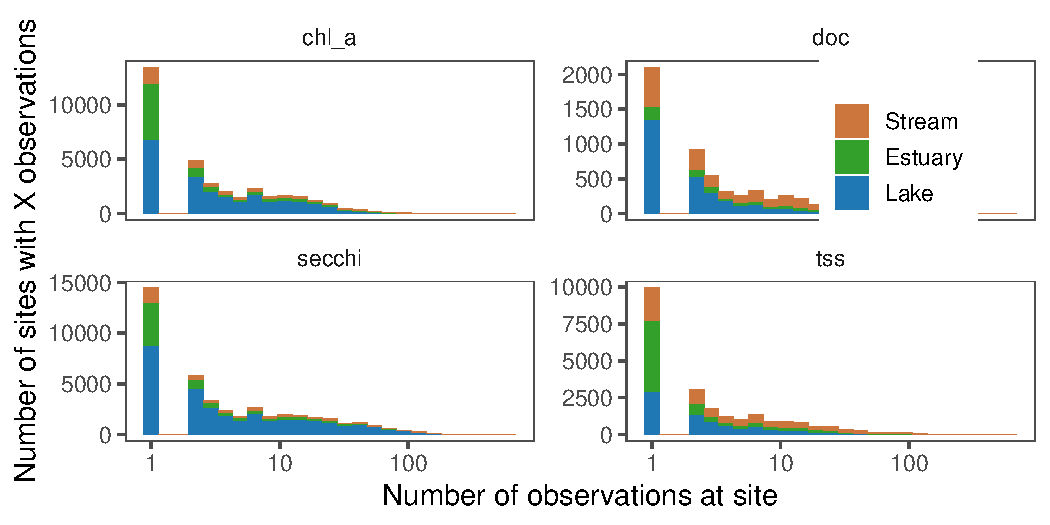
\includegraphics{aquasat_outline_files/figure-latex/distribution-1.pdf}
\caption{\label{fig:distribution} Shows the distribution of observations
at a given site. Most sites only have a single overpass observation, but
there are thousands of these sites}
\end{figure}

The timing of Observations in our matchup dataset generally reflect the
availability of data in the WQP and LAGOS-NE and the launching or
retirement of Landsat missions (Fig \ref{fig:time}). The data shown here
lines up well with data reported in the original WQP data paper (E. K.
Read et al. 2017). As with fig \ref{fig:distribution}, there is
consistently relatively low amounts of DOC data available throughout the
observation record with much more TSS, Chl.a, and secchi depth
information, especially in the years from 1999-2012.

\begin{figure}
\centering
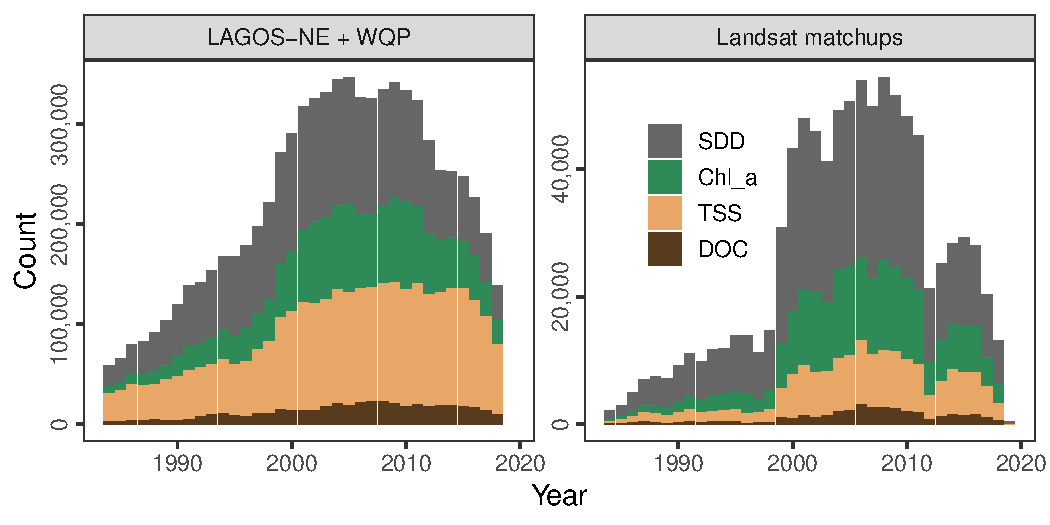
\includegraphics{aquasat_outline_files/figure-latex/time-1.pdf}
\caption{\label{fig:time} Shows the number of observations per year per
parameter type. Notice the continued increase in available data in
LAGOS-NE and the WQP through \textasciitilde{} 2010, with a decline in
data thereafter. This decline may reflect a lag between agencies
collecting data and submitting final datasets to the WQP. The matchup
data reflects the in-situ data while also showing peaks in overpasses
when at least two Landsat satellites are in orbit (late 1990s and
post-2013).}
\end{figure}

The data we captured in the matchup dataset generally reflects the
distribution of \emph{in-situ} data quite well (fig \ref{fig:captured}).
This is especially true for chlorophyll a and secchi disk depth, where
the overpass distribution shapes are nearly identical to the
\emph{in-situ} distributions, with just fewer observations. In both DOC
and TSS data, the matchup data misses the long tails of these
distributions (the highest TSS data and the highest and lowest DOC
data). If we examine which sites are missing in the overpass dataset, we
see that almost all of them are small streams, reflecting higher
variation in TSS and DOC in small streams that gets muted as small
stream signals mix to form larger river, more muted signals
({\textbf{???}}). For all parameters the observations captured span
several orders of magnitude and capture environmentally meaningful
variation in water clarity and quality. Across all parameters the data
is approximately log-normally distributed, with the majority of the data
occuring in narrow ranges for each parameter (fig \ref{fig:captured}).
Across all parameters the bottom 5 and the top 95th percentiles capture
more variation in concentratnoi than the 5-95\% quantiles, reflecting a
dataset that does capture large variation, but where the majority of
observations are restricted to narrow bands. \emph{ECOREGION BREAKDOWN
OF THIS?}

\begin{figure}
\centering
\includegraphics{aquasat_outline_files/figure-latex/captured-1.pdf}
\caption{\label{fig:captured} data distributions with quantile
breakdown}
\end{figure}

More stuff means more reflectance.

\includegraphics{aquasat_outline_files/figure-latex/variation-1.pdf}

\section{Discussion}\label{discussion}

\begin{center}\rule{0.5\linewidth}{\linethickness}\end{center}

\section*{References}\label{references}
\addcontentsline{toc}{section}{References}

\hypertarget{refs}{}
\hypertarget{ref-Blondeau-Patissier2014}{}
Blondeau-Patissier, David, James F.R. Gower, Arnold G. Dekker, Stuart R.
Phinn, and Vittorio E. Brando. 2014. ``A review of ocean color remote
sensing methods and statistical techniques for the detection, mapping
and analysis of phytoplankton blooms in coastal and open oceans.''
\emph{Progress in Oceanography} 123. Elsevier Ltd: 23--144.
doi:\href{https://doi.org/10.1016/j.pocean.2013.12.008}{10.1016/j.pocean.2013.12.008}.

\hypertarget{ref-Bukata2013}{}
Bukata, Robert P. 2013. ``Retrospection and introspection on remote
sensing of inland water quality: `Like Déjà Vu All Over Again'.''
Elsevier B.V.
doi:\href{https://doi.org/10.1016/j.jglr.2013.04.001}{10.1016/j.jglr.2013.04.001}.

\hypertarget{ref-Butman2016}{}
Butman, David, Sarah Stackpoole, Edward Stets, Cory P. McDonald, David
W. Clow, and Robert G. Striegl. 2016. ``Aquatic carbon cycling in the
conterminous United States and implications for terrestrial carbon
accounting.'' \emph{Proceedings of the National Academy of Sciences} 113
(1): 58--63.
doi:\href{https://doi.org/10.1073/pnas.1512651112}{10.1073/pnas.1512651112}.

\hypertarget{ref-Clarke1970}{}
Clarke, G. L., G. C. Ewing, and C. J. Lorenzen. 1970. ``Spectra of
Backscattered Light from the Sea Obtained from Aircraft as a Measure of
Chlorophyll Concentration.'' \emph{Science} 167 (3921): 1119--21.
doi:\href{https://doi.org/10.1126/science.167.3921.1119}{10.1126/science.167.3921.1119}.

\hypertarget{ref-Feldman1979}{}
Feldman, Stuart I. 1979. ``Make --- a program for maintaining computer
programs.'' \emph{Software: Practice and Experience} 9 (4): 255--65.
doi:\href{https://doi.org/10.1002/spe.4380090402}{10.1002/spe.4380090402}.

\hypertarget{ref-Gholizadeh2016}{}
Gholizadeh, Mohammad, Assefa Melesse, and Lakshmi Reddi. 2016. ``A
Comprehensive Review on Water Quality Parameters Estimation Using Remote
Sensing Techniques.'' \emph{Sensors} 16 (8): 1298.
doi:\href{https://doi.org/10.3390/s16081298}{10.3390/s16081298}.

\hypertarget{ref-Gorelick2017}{}
Gorelick, Noel, Matt Hancher, Mike Dixon, Simon Ilyushchenko, David
Thau, and Rebecca Moore. 2017. ``Google Earth Engine: Planetary-scale
geospatial analysis for everyone.'' \emph{Remote Sensing of Environment}
202 (December): 18--27.
doi:\href{https://doi.org/10.1016/j.rse.2017.06.031}{10.1016/j.rse.2017.06.031}.

\hypertarget{ref-Griffin2011}{}
Griffin, Claire G., Karen E. Frey, John Rogan, and Robert M. Holmes.
2011. ``Spatial and interannual variability of dissolved organic matter
in the Kolyma River, East Siberia, observed using satellite imagery.''
\emph{Journal of Geophysical Research: Biogeosciences} 116 (3): 1--12.
doi:\href{https://doi.org/10.1029/2010JG001634}{10.1029/2010JG001634}.

\hypertarget{ref-Holyer1978}{}
Holyer, Ronald J. 1978. ``Toward universal multispectral suspended
sediment algorithms.'' \emph{Remote Sensing of Environment} 7 (4):
323--38.
doi:\href{https://doi.org/10.1016/0034-4257(78)90023-8}{10.1016/0034-4257(78)90023-8}.

\hypertarget{ref-Klemas1973}{}
Klemas, V., J. F. Borchardt, and W. M. Treasure. 1973. ``Suspended
sediment observations from ERTS-1.'' \emph{Remote Sensing of
Environment} 2: 205--21.
doi:\href{https://doi.org/10.1016/0034-4257(71)90094-0}{10.1016/0034-4257(71)90094-0}.

\hypertarget{ref-Loveland2012}{}
Loveland, Thomas R., and John L. Dwyer. 2012. ``Landsat: Building a
strong future.'' \emph{Remote Sensing of Environment} 122 (October
2000). Elsevier B.V.: 22--29.
doi:\href{https://doi.org/10.1016/j.rse.2011.09.022}{10.1016/j.rse.2011.09.022}.

\hypertarget{ref-Maul1975}{}
Maul, George A., and Howard R. Gordon. 1975. ``On the Use of the Earth
Resources Technology Satellite ( LANDSAT-1 ) in Optical Oceanography.''
\emph{Remote Sensing of Environment} 4 (C): 95--128.
doi:\href{https://doi.org/10.1016/0034-4257(75)90008-5}{10.1016/0034-4257(75)90008-5}.

\hypertarget{ref-Olmanson2011}{}
Olmanson, Leif G., Patrick L. Brezonik, and Marvin E. Bauer. 2011.
``Evaluation of medium to low resolution satellite imagery for regional
lake water quality assessments.'' \emph{Water Resources Research} 47
(9): 1--14.
doi:\href{https://doi.org/10.1029/2011WR011005}{10.1029/2011WR011005}.

\hypertarget{ref-Pekel2016}{}
Pekel, Jean-François, Andrew Cottam, Noel Gorelick, and Alan S. Belward.
2016. ``High-resolution mapping of global surface water and its
long-term changes.'' \emph{Nature} 540 (7633). Nature Publishing Group:
418--22.
doi:\href{https://doi.org/10.1038/nature20584}{10.1038/nature20584}.

\hypertarget{ref-Read2017}{}
Read, Emily K., Lindsay Carr, Laura De Cicco, Hilary A Dugan, Paul C
Hanson, Julia A Hart, James Kreft, Jordan S Read, and Luke A Winslow.
2017. ``Water quality data for national-scale aquatic research: The
Water Quality Portal.'' \emph{Water Resources Research} 53 (2):
1735--45.
doi:\href{https://doi.org/10.1002/2016WR019993}{10.1002/2016WR019993}.

\hypertarget{ref-Ritchie1976}{}
Ritchie, JC, FR Schiebe, and JR McHENRY. 1976. ``Remote sensing of
suspended sediments in surface waters.'' \emph{American Society of} 42
(12): 1539--45. \url{https://trid.trb.org/view.aspx?id=66674}.

\hypertarget{ref-Soranno2017}{}
Soranno, Patricia A., Linda C. Bacon, Michael Beauchene, Karen E.
Bednar, Edward G. Bissell, Claire K. Boudreau, Marvin G. Boyer, et al.
2017. ``LAGOS-NE: A multi-scaled geospatial and temporal database of
lake ecological context and water quality for thousands of US lakes.''
\emph{GigaScience} 6 (12): 1--22.
doi:\href{https://doi.org/10.1093/gigascience/gix101}{10.1093/gigascience/gix101}.

\hypertarget{ref-Sprague2017}{}
Sprague, Lori A., Gretchen P. Oelsner, and Denise M. Argue. 2017.
``Challenges with secondary use of multi-source water-quality data in
the United States.'' \emph{Water Research} 110. Elsevier Ltd: 252--61.
doi:\href{https://doi.org/10.1016/j.watres.2016.12.024}{10.1016/j.watres.2016.12.024}.

\hypertarget{ref-Stets2012}{}
Stets, Edward G., and Robert G. Strieg. 2012. ``Carbon export by rivers
draining the conterminous united states.'' \emph{Inland Waters} 2 (4):
177--84.
doi:\href{https://doi.org/10.5268/IW-2.4.510}{10.5268/IW-2.4.510}.

\hypertarget{ref-Torbick2013}{}
Torbick, Nathan, Sarah Hession, Stephen Hagen, Narumon Wiangwang, Brian
Becker, and Jiaguo Qi. 2013. ``Mapping inland lake water quality across
the Lower Peninsula of Michigan using Landsat TM imagery.''
doi:\href{https://doi.org/10.1080/01431161.2013.822602}{10.1080/01431161.2013.822602}.

\hypertarget{ref-Wickham2014}{}
Wickham, Hadley. 2014. ``Tidy Data.'' \emph{Journal of Statistical
Software} 59 (10).
doi:\href{https://doi.org/10.18637/jss.v059.i10}{10.18637/jss.v059.i10}.

\hypertarget{ref-Wulder2016}{}
Wulder, Michael A., Joanne C. White, Thomas R. Loveland, Curtis E.
Woodcock, Alan S. Belward, Warren B. Cohen, Eugene A. Fosnight, Jerad
Shaw, Jeffrey G. Masek, and David P. Roy. 2016. ``The global Landsat
archive: Status, consolidation, and direction.'' \emph{Remote Sensing of
Environment} 185. Elsevier B.V.: 271--83.
doi:\href{https://doi.org/10.1016/j.rse.2015.11.032}{10.1016/j.rse.2015.11.032}.


\end{document}
